\documentclass[border=5mm]{standalone}
\usepackage{pgfplots}
\begin{document}

    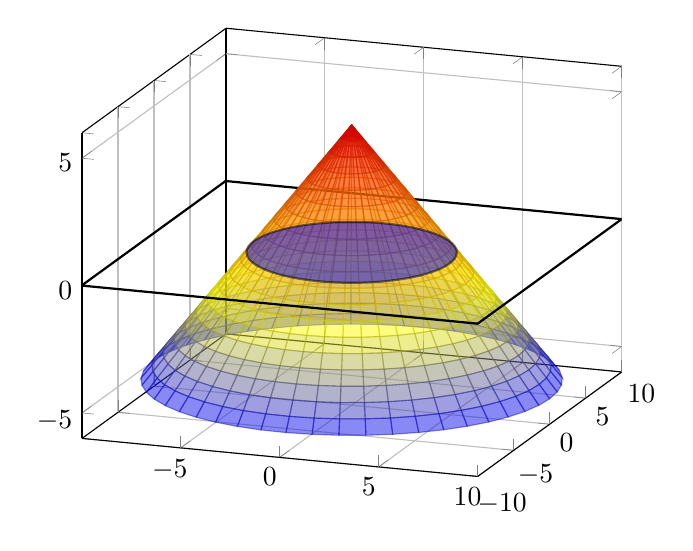
\begin{tikzpicture}
    \begin{axis}[grid=major,view={20}{20},z buffer=sort, data cs=polar]
   	\draw[thick] (axis cs:-10,10,0) -- (axis cs:10,10,0);
      \addplot3 [surf, domain=0:360,domain y=0:10,samples=50, samples y=20,opacity=0.5]{-y+5};
      	\draw[thick]  (axis cs:-10,10,0) -- (axis cs:-10,-10,0) -- (axis cs:10,-10,0) -- (axis cs:10,10,0);
	\draw[thick,fill=blue,opacity=0.5] (axis cs:0,0,0) ellipse [x radius=1.1em, y radius=3.8em, rotate=90];
           \end{axis}
  \end{tikzpicture} 



    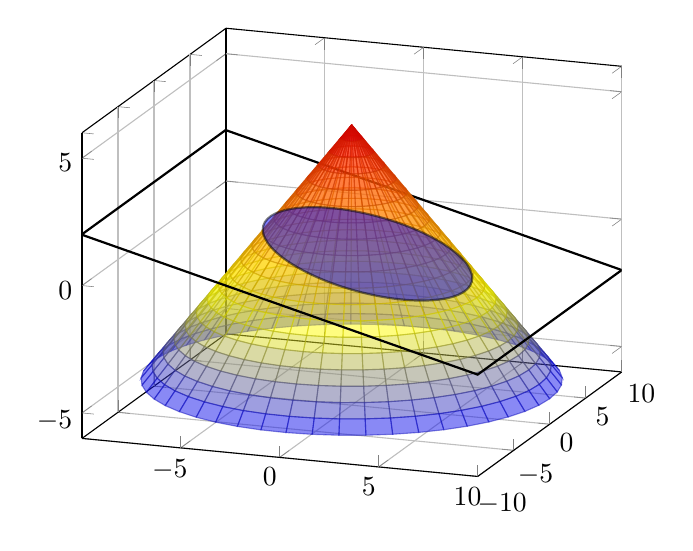
\begin{tikzpicture}
    \begin{axis}[grid=major,view={20}{20},z buffer=sort, data cs=polar]
   	\draw[thick] (axis cs:-10,10,2) -- (axis cs:10,10,-2);
      \addplot3 [surf, domain=0:360,domain y=0:10,samples=50, samples y=20,opacity=0.5]{-y+5};
      	\draw[thick]  (axis cs:-10,10,2) -- (axis cs:-10,-10,2) -- (axis cs:10,-10,-2) -- (axis cs:10,10,-2);
	\draw[thick,fill=blue,opacity=0.5] (axis cs:+0.8,0,0) ellipse [x radius=1.4em, y radius=3.9em, rotate=75];
           \end{axis}
  \end{tikzpicture} 

  
  
\end{document}